\chapter{arrows箭头}
箭头除了最普通的那种以外,其他的需要加载\texinline{arrows.meta}库,以前的\texinline{arrows}\texinline{arrows.space}已经过时。另外新的功能强大的箭头的命名规则是首字母大写。
\begin{texlst}
	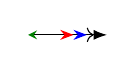
\begin{tikzpicture}
		\draw[{stealth[green!50!black]}-{Stealth[red]Stealth[blue]>Latex}] (0,0) -- (1,0);
	\end{tikzpicture}
\end{texlst}
路径上可以有多个箭头。

\section{箭头显示的规则}
\texinline{tips}可以设置了\forcsvlist{\texinline}{true, proper, on draw, on proper draw, never or
	false},以下一些示例可以说明显示箭头与否的规则:
\begin{texlst}
	\begin{tikzpicture}
		\matrix[row sep=1em, column sep=1em]{
			\node[circle, draw]{1}; & \draw [<->];                                           \\ %没有路径,所以没有箭头
			\node[circle, draw]{2}; & \draw [<->] (0,0);                                     \\ %因为没有路径,所以箭头退化
			\node[circle, draw]{3}; & \draw [<->, tips=proper] (0,0);                        \\ %proper选项抑制箭头显示
			\node[circle, draw]{4}; & \draw [<->] (0,0) -- (1,0);                            \\ %正常情况
			\node[circle, draw]{5}; & \draw [<->] (0,0) -- (1,0) (2, 0) -- (3, 0);           \\ %有两个子路径,只有最后一个有箭头
			\node[circle, draw]{6}; & \draw [<->] (0,0) -- (1,0) (2,0);                      \\%第二个子路径退化,所以箭头也退化
			\node[circle, draw]{7}; & \draw [<->, tips=on proper draw] (0,0) -- (1,0) (2,0); \\%第二个子路径退化,但是on proper draw抑制箭头显示
			\node[circle, draw]{8}; & \draw [<->] (0,0) circle[radius=2pt] (2,0) -- (3,0);   \\%有两个子路径,但是其中一个是封闭的,所以不显示任何箭头
		};
	\end{tikzpicture}
\end{texlst}

\section{箭头的外观}
\subsection{尺寸}
\texinline{length}选项可以设置箭头的长度,如:
\begin{texlst}
	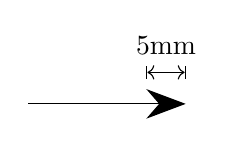
\begin{tikzpicture}
		\draw [-{Stealth[length=5mm]}] (0,0) -- (2,0);
		\draw [|<->|] (1.5,0.4) -- node[above=1mm]{5mm} (2,0.4);
	\end{tikzpicture}
\end{texlst}

还有一种标识方法,\texinline{length=3pt 5},其中5是倍数,基数是标准线的宽度$0.4pt$,$0.4pt \times 5 + 3pt = 5pt$。

另外,在双线模式下才生效,写做\texinline{length=0pt 3 0}样式,其中的第三个参数称为线宽因子(Line Width
Factors)。其计算公式如下:
\begin{align*}
	\omega   & = \langle outer factor\rangle\omega_0 + (1-\langle outer factor\rangle )\omega_t \\
	\omega_0 & 双线的线宽                                                                            \\
	\omega_t & 双线的总线宽
\end{align*}

下面来看三个示例:
\begin{texlst}
	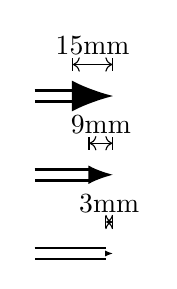
\begin{tikzpicture}
		\draw [line width=1pt, double distance=3pt, arrows={-Latex[length=0pt 3 0]}] (0,0) -- (1,0);
		\draw[|<->|] (1cm-15pt, 0.4) --node[above] {15mm} (1,0.4);
		% 1pt * 0 + (1-0) * 5 = 5 * 3 = 15pt
		\draw [yshift=-1cm, line width=1pt, double distance=3pt, arrows={-Latex[length=0pt 3 0.5]}] (0,0) -- (1,0);
		% 1pt * 0.5 + (1-0.5) * 5 = 3 * 3 = 9pt
		\draw[|<->|, yshift=-1cm] (1cm-9pt, 0.4) --node[above] {9mm} (1,0.4);
		\draw [yshift=-2cm, line width=1pt, double distance=3pt, arrows={-Latex[length=0pt 3 1]}] (0,0) -- (1,0);
		% 1pt * 1 + (1-1) * 5 = 1 * 3 = 3pt
		\draw[|<->|, yshift=-2cm] (1cm-3pt, 0.4) --node[above] {3mm} (1,0.4);
	\end{tikzpicture}
\end{texlst}

\texinline{length}和\texinline{width}可以分别设置箭头的长度和宽度。另外还有一个\texinline{width'}选项,设置的格式为\\
\texinline{width'=0pt .5}, 这个写法的意思是宽度是其长度的一半。

\begin{texlst}
	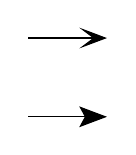
\begin{tikzpicture}
		\draw [arrows={-Stealth[length=10pt, inset=5pt]}] (0,0) -- (1,0);
		\draw [arrows={-Stealth[length=10pt, inset=2pt]}, yshift=-1cm] (0,0) -- (1,0);
	\end{tikzpicture}
\end{texlst}

另外,\texinline{inset'}选项跟\texinline{width'}一样,可以设置\texinline{inset}与长度的倍数关系。

\texinline{angle}用来设置箭头的角度,并且角度后面也可以附带设置箭头的长度。如下例:
\begin{texlst}
	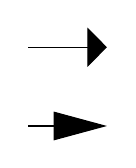
\begin{tikzpicture}
		\draw [arrows={-Stealth[inset=0pt, angle=90:10pt]}] (0,0) -- (1,0);
		\draw [yshift=-1cm, arrows={-Stealth[inset=0pt, angle=30:20pt]}] (0,0) -- (1,0);
	\end{tikzpicture}
\end{texlst}

\subsection{缩放}
用\texinline{scale}选项可以设置缩放比例,如下例:
\begin{texlst}
	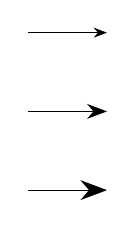
\begin{tikzpicture}
		\draw [arrows={-Stealth[]}] (0,1) -- (1,1);
		\draw [arrows={-Stealth[scale=1.5]}, yshift=-1cm] (0,1) -- (1,1);
		\draw [arrows={-Stealth[scale=2]}, yshift=-2cm] (0,1) -- (1,1);
	\end{tikzpicture}
\end{texlst}

另外还有长度和宽度分别缩放的选项\texinline{length scale}和\texinline{width scale}:
\begin{texlst}
	\begin{tikzpicture}
		\draw [arrows={-Stealth[]}] (0,1) -- (1,1);
		\draw [arrows={-Stealth[scale length=1.5]}, yshift=-1cm] (0,1) -- (1,1);
		\draw [arrows={-Stealth[scale length=2]}, yshift=-2cm] (0,1) -- (1,1);
	\end{tikzpicture}
\end{texlst}
\begin{texlst}
	\begin{tikzpicture}
		\draw [arrows={-Stealth[]}] (0,1) -- (1,1);
		\draw [arrows={-Stealth[scale width=1.5]}, yshift=-1cm] (0,1) -- (1,1);
		\draw [arrows={-Stealth[scale width=2]}, yshift=-2cm] (0,1) -- (1,1);
	\end{tikzpicture}
\end{texlst}

\texinline{arc}选项用来设置箭头中弧形部分:
\begin{texlst}
	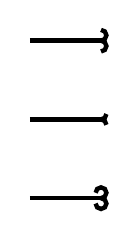
\begin{tikzpicture}[ultra thick]
		\draw [arrows={-Hooks[]}] (0,0) -- (1,0);
		\draw [yshift=-1cm, arrows={-Hooks[arc=90]}] (0,0) -- (1,0);
		\draw [yshift=-2cm, arrows={-Hooks[arc=270]}] (0,0) -- (1,0);
	\end{tikzpicture}
\end{texlst}

\texinline{slant}选项用来设置倾斜:
\begin{texlst}
	\begin{tikzpicture}
		\draw [arrows = {->[]}] (0,0) -- (1,0);
		\draw [yshift=-1cm, arrows = {->[slant=0.5]}] (0,0) -- (1,0);
		\draw [yshift=-2cm, arrows = {->[slant=1]}] (0,0) -- (1,0);
	\end{tikzpicture}
\end{texlst}

\texinline{reversed}选项用来反向箭头,并且如果反向两次可以还原:
\begin{texlst}
	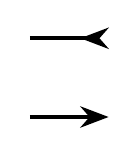
\begin{tikzpicture}[ultra thick]
		\draw  [arrows = {-Stealth[reversed]}] (0,0) -- (1,0);
		\draw  [yshift=-1cm, arrows = {-Stealth[reversed, reversed]}] (0,0) -- (1,0);
	\end{tikzpicture}
\end{texlst}

\texinline{harpoon}、\texinline{swap}配合起来实现箭头的左半或右半:
\begin{texlst}
	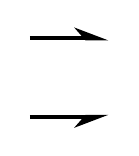
\begin{tikzpicture}[ultra thick]
		\draw [arrows={-Stealth[harpoon]}] (0,0) -- (1,0);
		\draw [yshift=-1cm, arrows={-Stealth[harpoon, swap]}] (0,0) -- (1,0);
	\end{tikzpicture}
\end{texlst}

\texinline{left}、\texinline{right}是上面两种方法的快捷方式:
\begin{texlst}
	\begin{tikzpicture}
		\draw [arrows={-Stealth[left]}] (0,0) -- (1,0);
		\draw [yshift=-1cm, arrows={-Stealth[right]}] (0,0) -- (1,0);
	\end{tikzpicture}
\end{texlst}

\section{颜色 Color}
同路径一样,箭头也可以设置颜色\texinline{color}及填充\texinline{fill}属性。\texinline{open}属性相当于\texinline{fill=none}。

\section{线条样式}
\subsection{箭头线条帽子 Line Cap}
与线条的类似,但是箭头线条帽子只有两种样式:\forcsvlist{\texinline}{round, butt},\texinline{rect}在这里是不合法的。
\begin{texlst}
	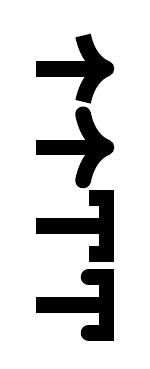
\begin{tikzpicture}[line width=2mm]
		\draw [arrows={-Computer Modern Rightarrow[line cap=butt]}] (0,0) -- (1,0);
		\draw [yshift=-1cm, arrows={-Computer Modern Rightarrow[line cap=round]}] (0,0) -- (1,0);
		\draw [yshift=-2cm, arrows={-Bracket[line cap=butt]}] (0,0) -- (1,0);
		\draw [yshift=-3cm, arrows={-Bracket[line cap=round]}] (0,0) -- (1,0);
	\end{tikzpicture}
\end{texlst}

\subsection{箭头连接 Line Join}
与线条类似,但是箭头连接也只有两种样式:\forcsvlist{\texinline}{round, miter},\texinline{bevel}不合法。
\begin{texlst}
	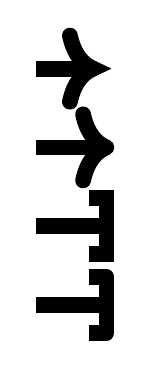
\begin{tikzpicture}[line width=2mm]
		\draw [arrows={-Computer Modern Rightarrow[line join=miter]}] (0,0) -- (1,0);
		\draw [yshift=-1cm, arrows={-Computer Modern Rightarrow[line join=round]}] (0,0) -- (1,0);
		\draw [yshift=-2cm, arrows={-Bracket[line join=miter]}] (0,0) -- (1,0);
		\draw [yshift=-3cm, arrows={-Bracket[line join=round]}] (0,0) -- (1,0);
	\end{tikzpicture}
\end{texlst}

\subsection{圆角 round}
\texinline{round}属性是\texinline{line cap=round, line join=round}的快捷方式。

\subsection{尖角 sharp}
\texinline{sharp}属性是\texinline{line cap=butt, line join=miter}的快捷方式。

\subsection{线宽 line width}
\texinline{line width}属性用于设置箭头的线宽。

\subsection{扭转伸缩 Beding and Flexing}
前面的全部是连接直线的情况,下面来看看复杂扭曲和伸缩的情况。
\begin{texlst}
	\def\wall{\fill [fill=black!50] (1,-0.5) rectangle (2, 0.5);
		\pattern [pattern=bricks] (1,-0.5) rectangle (2,0.5);
		\draw [line width=1pt] (1cm+0.5pt, -0.5) -- ++(0,1);}
	\begin{tikzpicture}
		\wall
		\draw [red!25, line width=1mm] (-1,0) -- (1,0);
		\draw [red, line width=1mm, -{Stealth[length=1cm, open, blue, quick]}] (-1,-.5) .. controls (0,-.5) and (0,0) .. (1,0);
	\end{tikzpicture}
\end{texlst}
我仔细对比了加\texinline{quick}选项与不加的效果,感觉没有什么区别。
用在一个箭头的情况没有问题,但是在下面的示例中,多个箭头就出问题了。
\begin{texlst}
	\def\wall{\fill [fill=black!50] (1,-0.5) rectangle (2, 0.5);
		\pattern [pattern=bricks] (1,-0.5) rectangle (2,0.5);
		\draw [line width=1pt] (1cm+0.5pt, -0.5) -- ++(0,1);}
	\begin{tikzpicture}
		\wall
		\draw [red!25, line width=1mm] (-1,0) -- (1,0);
		\draw [red, line width=1mm, -{[quick, sep]>>>}] (-1,-.5) .. controls (0,-.5) and (0,0) .. (1,0);
	\end{tikzpicture}
\end{texlst}
这里就开始需要\texinline{bending}库出场了。

\texinline{flex}、\texinline{bend}需要加载\texinline{beding}库。\texinline{flex}以及\texinline{flex'}选项效果一般,我看还不如\texinline{quick
	and dirty},但是\texinline{bend}选项就不一样了,感觉很流畅。
\begin{texlst}
	\usetikzlibrary{arrows.meta, bending}
	\def\wall{\fill [fill=black!50] (1,-0.5) rectangle (2, 0.5);
		\pattern [pattern=bricks] (1,-0.5) rectangle (2,0.5);
		\draw [line width=1pt] (1cm+0.5pt, -0.5) -- ++(0,1);}
	\begin{tikzpicture}
		\wall
		\draw [red!25, line width=1mm] (-1,0) -- (1,0);
		\draw [red, line width=1mm, -{Stealth[length=20pt, bend]}] (-1,-.5) .. controls (0,-.5) and (0,0) .. (1,0);
	\end{tikzpicture}
\end{texlst}

而且在多个箭头的情况下也表现很自然。
\begin{texlst}
	\usetikzlibrary{bending}
	\def\wall{\fill [fill=black!50] (1,-0.5) rectangle (2, 0.5);
		\pattern [pattern=bricks] (1,-0.5) rectangle (2,0.5);
		\draw [line width=1pt] (1cm+0.5pt, -0.5) -- ++(0,1);}
	\begin{tikzpicture}
		\wall
		\draw [red!25, line width=1mm] (-1,0) -- (1,0);
		\draw [red, line width=1mm, -{[bend, sep]>>>}] (-1,-.5) .. controls (0,-.5) and (0,0) .. (1,0);
	\end{tikzpicture}
\end{texlst}

\section{箭头规格}
\subsection{箭头间距 sep}
\begin{texlst}
	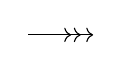
\begin{tikzpicture}
		\draw[-{>[sep=1pt]>[sep=2pt]>[sep=5pt]}] (0,1) -- (1,1);
	\end{tikzpicture}
\end{texlst}

\subsection{明确线端}
\begin{texlst}
	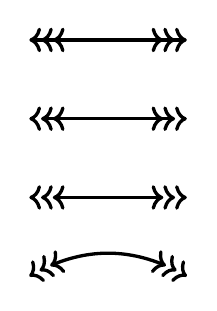
\begin{tikzpicture}
		\draw[very thick, <<<->>>] (0,0) -- (2,0);
		\draw[very thick, <.<<->>.>, yshift=-1cm] (0,0) -- (2,0);
		\draw[very thick, <<.<->.>>, yshift=-2cm] (0,0) -- (2,0);
		\draw[very thick, <<.<->.>>, yshift=-3cm] (0,0) to[bend left] (2,0);
	\end{tikzpicture}
\end{texlst}

\subsection{定义箭头快捷方式}
\begin{texlst}
	\begin{tikzpicture}[myarrow/.tip= {Stealth[sep]. >>}]
		\draw[-myarrow] (0,0) -- (2,0);
	\end{tikzpicture}
\end{texlst}

\subsection{>=}
用来设置箭头样式。

\subsection{shorten >=/<=}
设置箭头与目标之间的空距。

\subsection{arrows}
用于设置范围内所有箭头的样式。

\subsection{箭头样式参考}
\begin{arrowexamples}
	\arrowexample Arc Barb[]
	\arrowexample Bar[]
	\arrowexample Bracket[]
	\arrowexample Hooks[]
	\arrowexample Parenthesis[]
	\arrowexample Straight Barb[]
	\arrowexample Tee Barb[]
\end{arrowexamples}

\begin{arrowexamples}
	\arrowexample Classical TikZ Rightarrow[]
	\arrowexample Computer Modern Rightarrow[]
	\arrowexampledouble Implies[]
	\arrowexample To[]
\end{arrowexamples}

\begin{arrowexamples}
	\arrowexample Circle[]
	\arrowexample Diamond[]
	\arrowexample Ellipse[]
	\arrowexample Kite[]
	\arrowexample Latex[]
	\arrowexample Latex[round]
	\arrowexample Rectangle[]
	\arrowexample Square[]
	\arrowexample Stealth[]
	\arrowexample Stealth[round]
	\arrowexample Triangle[]
	\arrowexample Turned Square[]
\end{arrowexamples}

\begin{arrowexamples}
	\arrowexample Circle[open]
	\arrowexample Diamond[open]
	\arrowexample Ellipse[open]
	\arrowexample Kite[open]
	\arrowexample Latex[open]
	\arrowexample Latex[round,open]
	\arrowexample Rectangle[open]
	\arrowexample Square[open]
	\arrowexample Stealth[open]
	\arrowexample Stealth[round,open]
	\arrowexample Triangle[open]
	\arrowexample Turned Square[open]
\end{arrowexamples}

\begin{arrowcapexamples}
	\arrowcapexample Butt Cap[]
	\arrowcapexample Fast Round[]
	\arrowcapexample Fast Triangle[]
	\arrowcapexample Round Cap[]
	\arrowcapexample Triangle Cap[]
\end{arrowcapexamples}

\begin{arrowexamples}
	\arrowexample Rays[]
	\arrowexample Rays[n=8]
\end{arrowexamples}

这一章的内容暂时先到这儿,文档的高级写法真的很迷人。但是现在还是有些看不懂,而且箭头的形状也太多,暂时我只需要了解一些简单的就可以了。
